\section{Graphs and Plots}

\LaTeX{} can create high-quality graphs\index{graphs} and plots\index{plots} using the \texttt{pgfplots}\index{pgfplots} package. Here are examples of different plot types commonly used in scientific papers.

\subsection{Line Plot}

Line plots are useful for showing trends over time or continuous data:

\begin{figure}[H]
    \centering
    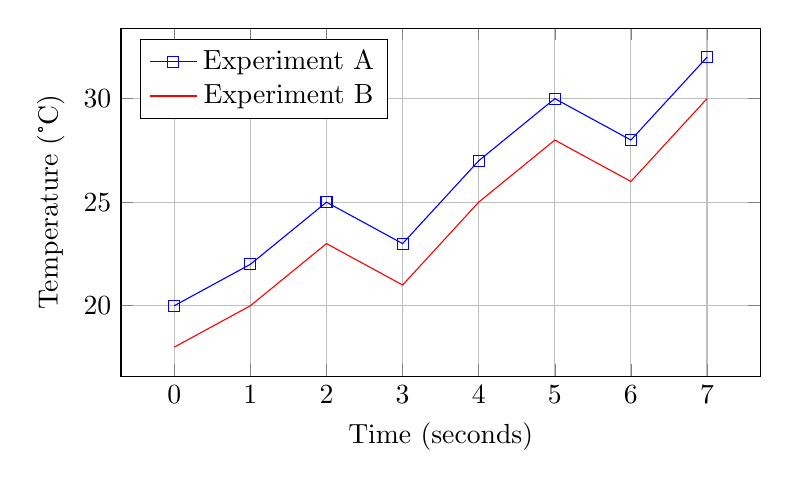
\begin{tikzpicture}
    \begin{axis}[
        xlabel={Time (seconds)},
        ylabel={Temperature (°C)},
        legend pos=north west,
        grid=major,
        width=0.8\textwidth,
        height=6cm
    ]
    \addplot[color=blue,mark=square] coordinates {
        (0,20) (1,22) (2,25) (3,23) (4,27) (5,30) (6,28) (7,32)
    };
    \addplot[color=red,mark=circle] coordinates {
        (0,18) (1,20) (2,23) (3,21) (4,25) (5,28) (6,26) (7,30)
    };
    \legend{Experiment A, Experiment B}
    \end{axis}
    \end{tikzpicture}
    \caption{Temperature measurements over time for two experiments.}
    \label{fig:lineplot}
\end{figure}

\subsection{Bar Chart}

Bar charts are ideal for comparing discrete categories:

\begin{figure}[H]
    \centering
    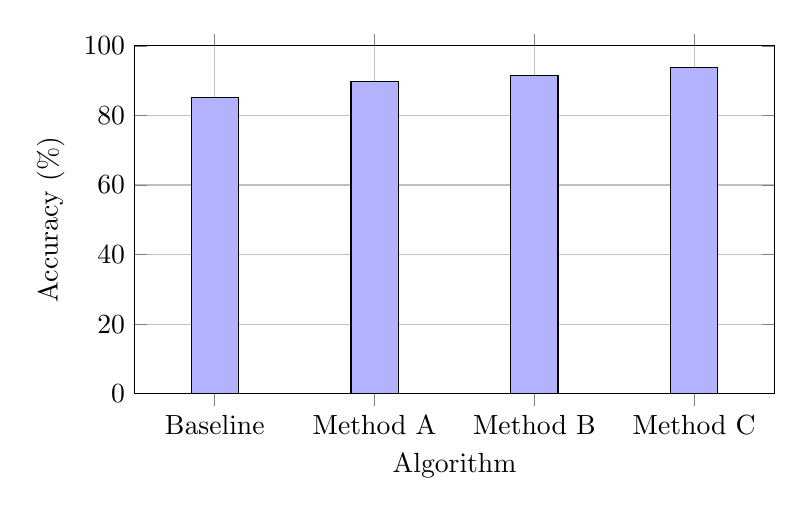
\begin{tikzpicture}
    \begin{axis}[
        ybar,
        bar width=0.6cm,
        xlabel={Algorithm},
        ylabel={Accuracy (\%)},
        xmin=-0.5,
        xmax=3.5,
        ymin=0,
        ymax=100,
        xtick=data,
        xticklabels={Baseline, Method A, Method B, Method C},
        grid=major,
        width=0.8\textwidth,
        height=6cm
    ]
    \addplot[fill=blue!30] coordinates {
        (0,85.2) (1,89.7) (2,91.4) (3,93.8)
    };
    \end{axis}
    \end{tikzpicture}
    \caption{Comparison of algorithm accuracy percentages.}
    \label{fig:barchart}
\end{figure}

\subsection{Scatter Plot}

Scatter plots show relationships between two variables:

\begin{figure}[H]
    \centering
    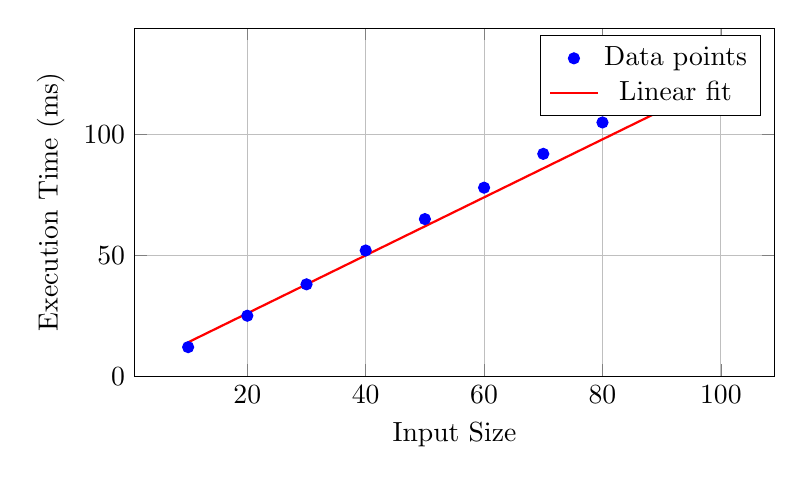
\begin{tikzpicture}
    \begin{axis}[
        xlabel={Input Size},
        ylabel={Execution Time (ms)},
        grid=major,
        width=0.8\textwidth,
        height=6cm
    ]
    \addplot[only marks,mark=*,mark size=2pt,color=blue] coordinates {
        (10,12) (20,25) (30,38) (40,52) (50,65) (60,78) (70,92) (80,105) (90,118) (100,132)
    };
    \addplot[color=red,thick,domain=10:100] {1.2*x + 2};
    \legend{Data points, Linear fit}
    \end{axis}
    \end{tikzpicture}
    \caption{Execution time versus input size with linear regression fit.}
    \label{fig:scatterplot}
\end{figure}

\subsection{Multiple Series Comparison}

Multiple data series can be compared in a single plot:

\begin{figure}[H]
    \centering
    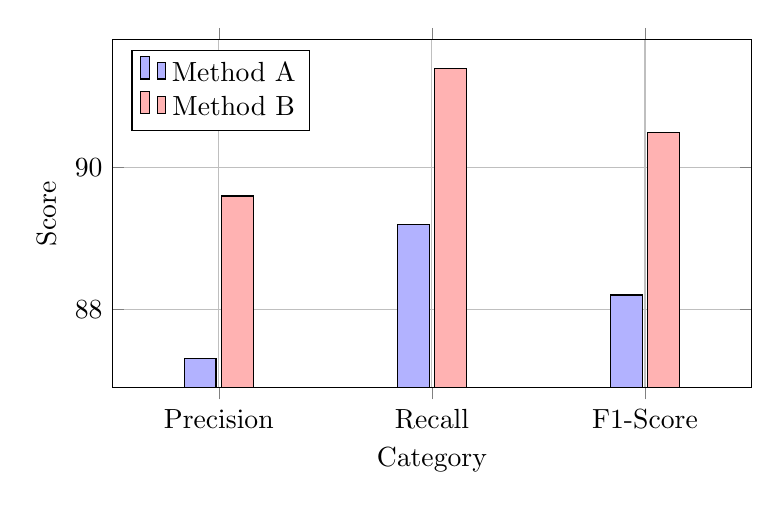
\begin{tikzpicture}
    \begin{axis}[
        ybar,
        bar width=0.4cm,
        xlabel={Category},
        ylabel={Score},
        xmin=-0.5,
        xmax=2.5,
        legend pos=north west,
        grid=major,
        width=0.8\textwidth,
        height=6cm,
        xtick=data,
        xticklabels={Precision, Recall, F1-Score}
    ]
    \addplot[fill=blue!30] coordinates {
        (0,87.3) (1,89.2) (2,88.2)
    };
    \addplot[fill=red!30] coordinates {
        (0,89.6) (1,91.4) (2,90.5)
    };
    \legend{Method A, Method B}
    \end{axis}
    \end{tikzpicture}
    \caption{Performance metrics comparison between two methods.}
    \label{fig:multibar}
\end{figure}

